\documentclass[12pt]{article}
\usepackage{graphicx}
\usepackage{amsmath}
\usepackage{geometry}
\geometry{a4paper, margin=1in}

\title{Data Communication Assignment: Multiplexing and Demultiplexing Techniques for Urban Communication Systems}
\author{}
\date{}

\begin{document}

\maketitle

\section*{Introduction}
In this assignment, we design a communication system for a densely populated urban area that supports multiple users simultaneously while ensuring efficient bandwidth utilization. The environment is prone to high electromagnetic interference due to numerous electronic devices. We discuss appropriate multiplexing and demultiplexing techniques, analyze their advantages and limitations, and propose strategies to handle interference and ensure reliable communication.

\section*{Multiplexing and Demultiplexing Techniques}
To address the challenges of the urban environment, we propose the use of \textbf{Orthogonal Frequency Division Multiplexing (OFDM)} combined with \textbf{Time Division Multiple Access (TDMA)}. These techniques are chosen based on their ability to handle interference, efficiently utilize bandwidth, and support multiple users.

\subsection*{Orthogonal Frequency Division Multiplexing (OFDM)}
OFDM divides the available bandwidth into multiple orthogonal subcarriers, each carrying a portion of the data. This technique is particularly effective in environments with high electromagnetic interference because:
\begin{itemize}
    \item It reduces inter-symbol interference (ISI) by using a guard interval.
    \item It allows efficient use of the spectrum by overlapping subcarriers without causing interference.
    \item It is robust against frequency-selective fading, which is common in urban areas.
\end{itemize}

\subsection*{Time Division Multiple Access (TDMA)}
TDMA divides time into slots and assigns each user a specific time slot for transmission. This ensures that multiple users can share the same frequency band without interference. TDMA complements OFDM by adding a temporal dimension to resource allocation.

\section*{Bandwidth Allocation Strategies}
To allocate bandwidth efficiently:
\begin{itemize}
    \item Use dynamic bandwidth allocation based on user demand and channel conditions.
    \item Prioritize critical applications (e.g., emergency services) by reserving specific subcarriers or time slots.
    \item Implement adaptive modulation and coding (AMC) to adjust data rates according to signal quality.
\end{itemize}

\section*{Handling Interference and Ensuring Reliability}
To mitigate interference and ensure reliable communication:
\begin{itemize}
    \item Employ error correction codes (e.g., Reed-Solomon or Turbo codes) to detect and correct errors caused by interference.
    \item Use frequency hopping spread spectrum (FHSS) to avoid persistent interference on specific frequencies.
    \item Implement power control mechanisms to minimize interference between users.
\end{itemize}

\section*{Diagram of OFDM-TDMA System}
Below is a diagram illustrating the proposed OFDM-TDMA system:

\begin{figure}[h]
    \centering
    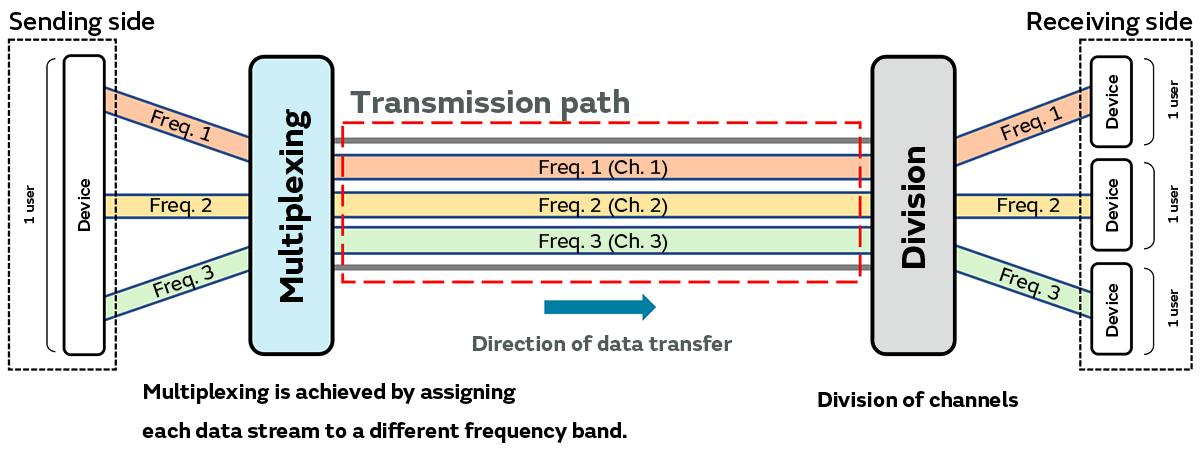
\includegraphics[width=1.0\textwidth]{./multiplex.png} % Replace with actual image file
    \caption{OFDM-TDMA Multiplexing Technique}
\end{figure}
\newpage
\section*{Advantages and Limitations of OFDM-TDMA}
\subsection*{Advantages}
\begin{itemize}
    \item Efficient use of bandwidth through orthogonal subcarriers and time slots.
    \item Robustness against interference and fading.
    \item Scalability to support a large number of users.
\end{itemize}

\subsection*{Limitations}
\begin{itemize}
    \item High computational complexity due to Fast Fourier Transform (FFT) operations in OFDM.
    \item Synchronization issues between users in TDMA.
    \item Sensitivity to Doppler effects in mobile environments.
\end{itemize}

\section*{Complex Problem-Solving Questions}
\begin{enumerate}
    \item \textbf{Does the solution need in-depth engineering knowledge?} \\
    Yes, the solution requires in-depth knowledge of communication systems, signal processing, and interference mitigation techniques.
    
    \item \textbf{Does the solution involve wide-ranging or conflicting technical, engineering, and other issues?} \\
    Yes, it involves balancing bandwidth efficiency, interference mitigation, and user fairness, which are often conflicting goals.
    
    \item \textbf{Is the solution well-known, or does it require abstract thinking and analysis to formulate?} \\
    While OFDM and TDMA are well-known, combining them effectively in an interference-prone urban environment requires abstract thinking and analysis.
    
    \item \textbf{Does the solution involve infrequently encountered issues?} \\
    Yes, the high level of electromagnetic interference and dense user population are challenging scenarios that are not commonly encountered.
    
    \item \textbf{Does the solution need adherence to standards and codes of practice?} \\
    Yes, compliance with communication standards (e.g., IEEE 802.11 for Wi-Fi) is essential.
    
    \item \textbf{Does the solution involve stakeholders with conflicting technical requirements?} \\
    Yes, different users may have conflicting requirements (e.g., high data rate vs. low latency).
    
    \item \textbf{Does the solution involve interdependence between sub-problems or parts?} \\
    Yes, interference mitigation, bandwidth allocation, and user scheduling are interdependent.
\end{enumerate}

\section*{Conclusion}
The proposed OFDM-TDMA system is well-suited for the given urban environment. It efficiently utilizes bandwidth, mitigates interference, and supports multiple users. However, careful implementation and optimization are required to address its limitations and ensure reliable communication.

\end{document}